\ifspanish

\question Considere un problema de decisión binaria unidimensional con verosimilitudes $p_{X|H}(x|h)$ y probabilidades a priori $P_H(h)$, con $h\in \{0,1\}$ y $P_H(1)=0.6$.
\begin{parts}
\part Se sabe que $P_{H|X}(h|x)=P_{H}(h)$, para $h\in \{0,1\}$ y para todo $x$. Determine el decisor MAP.
\part ¿Cuál es la probabilidad de error del decisor obtenido en el apartado anterior?
\part Ignore ahora la condición del apartado (a). Por contra, se sabe que las verosimilitudes son simétricas una de otra, es decir, $p_{X|H}(x|1)=p_{X|H}(-x|0)$. \textcolor{blue}{Determine un valor del umbral $\mu$ que garantice que el decisor de la forma
\begin{equation}
x \dunodcero \mu  \nonumber
\end{equation}
verifica $P_{FA}=P_{M}$.}
% ¿Cuál es el valor de $\mu$?.
\part Proponga, mediante una fórmula o un dibujo, un ejemplo de verosimilitudes simétricas (como en el apartado anterior) para las que el decisor ML no es de tipo umbral, es decir, no puede expresarse en la forma
\begin{equation}
x \dunodcero \alpha   \nonumber
\end{equation}
\end{parts}
\begin{solution}
\begin{parts}
\part	Siempre se decide $D=1$.
\part $P_{\rm e}=0.4 $
\part $\mu=0$
\part $ $\\
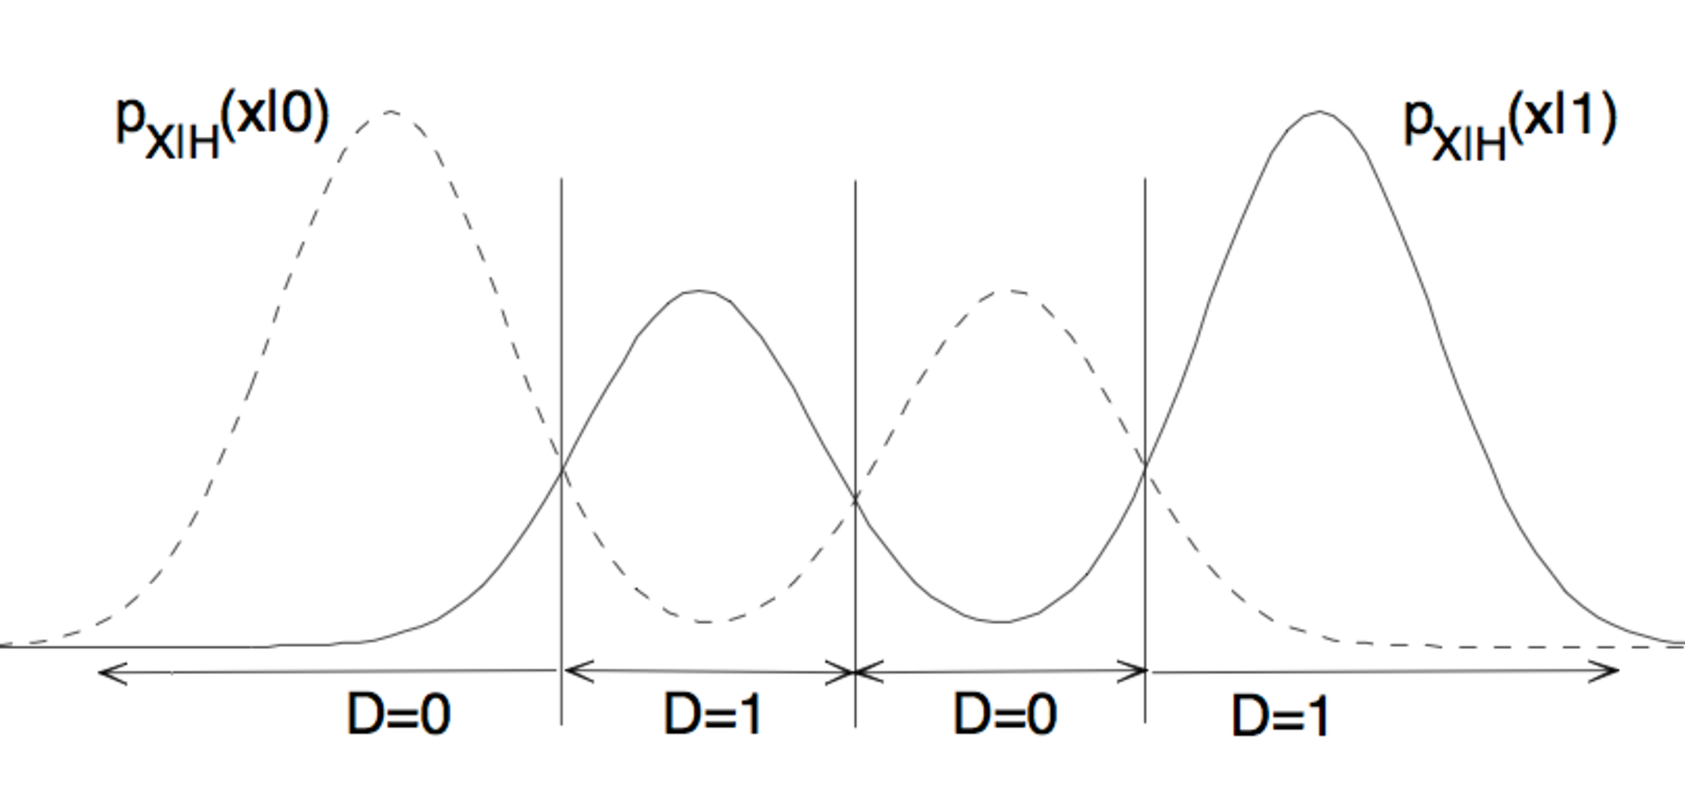
\includegraphics[width=8cm]{Figuras/genera_dist_bimodal.pdf}

\end{parts}
\end{solution}

\else

\question Consider a unidimensional binary decision problem with likelihoods $p_{X|H}(x|h)$ and {\em a priori} probabilities $P_H(h)$, with $h\in \{0,1\}$ and $P_H(1)=0.6$.
\begin{parts}
\part It is known that $P_{H|X}(h|x)=P_{H}(h)$, for $h\in \{0,1\}$, and for all $x$. Determine the MAP classifier.
\part Which is the probability of error of the decision maker obtained in the previous section?
\part Ignore now the condition of section (a). Instead, it is kwnon that the likelihoods are symmetric to each other, i.e.,  $p_{X|H}(x|1)=p_{X|H}(-x|0)$, and that some decision maker given by
\begin{equation}
x \dunodcero \mu  \nonumber
\end{equation}
verifies $P_{FA}=P_{M}$. Which is the value of $\mu$?.
\part Using an equation or a plot, propose and example of symmetric likelihoods (like in the previous section) for which the ML classifier is not a threshold decision maker, i.e., the ML classifier cannot be expressed as
\begin{equation}
x \dunodcero \alpha   \nonumber
\end{equation}
\end{parts}

\begin{solution}
\begin{parts}
\part The MAP classifier always selects $D=1$.
\part $P_{\rm e}=0.4 $
\part $\mu=0$
\part $ $\\
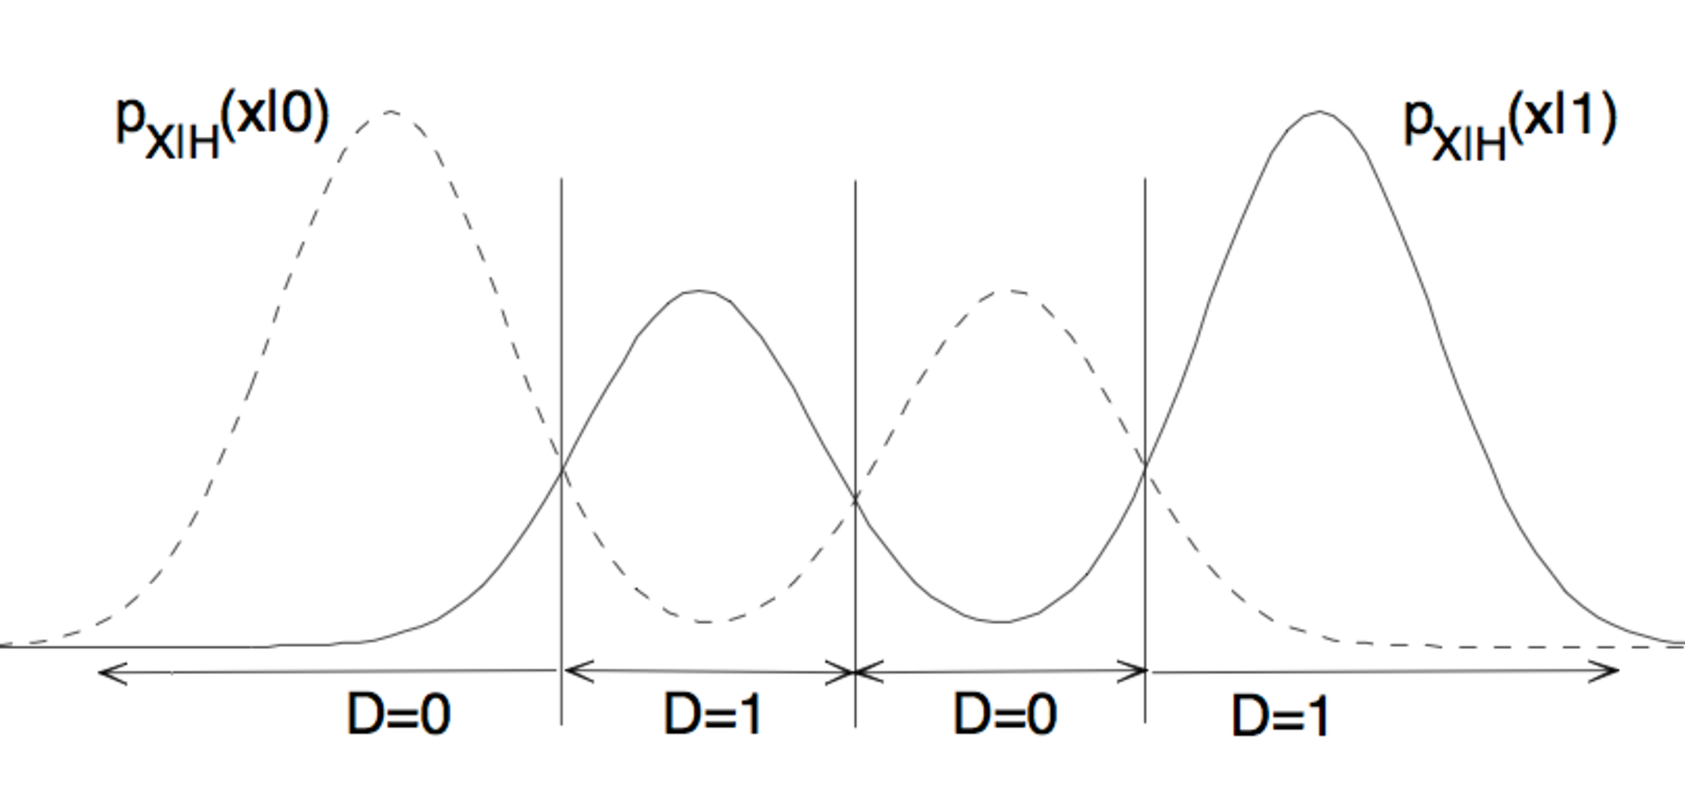
\includegraphics[width=8cm]{Figuras/genera_dist_bimodal.pdf}

\end{parts}
\end{solution}

\fi